\documentclass[a4paper,12pt]{article}

% Packages
\usepackage{float}
\usepackage[utf8]{inputenc}
\usepackage{fancyhdr}
\usepackage[left = 0.6 in, right = 0.6 in, top = 1 in, bottom = 1 in, headsep = 0.5 in]{geometry}
\usepackage[normalem]{ulem}
\usepackage{enumerate}
\usepackage{pgfplots}
\usepackage{titling}
\pgfplotsset{width=8cm,compat=1.9}
\usepackage{stackengine}
%\pagenumbering{gobble}
\usepackage[fleqn]{amsmath}
\usepackage{amssymb}
\usepackage[T1]{fontenc}
\usepackage{fancybox}
\usepackage{longtable}

\hfuzz = 100pt

%%% Horizontal Line Command
\makeatletter
  \newcommand*\variableheghtrulefill[1][.4\p@]{%
    \leavevmode
    \leaders \hrule \@height #1\relax \hfill
    \null
  }
\makeatother
%%%

%%% Header & Footer
\fancyhf{}
\renewcommand{\footrulewidth}{0.1mm}
\fancyhead[L]{Matteo Esposito, William Ngo, Spyros Orfanos, Frederic Siino}
%\fancyhead[C]{Assignment 1}
\fancyhead[R]{STAT 497-H}
%\fancyfoot[L]{ID: 40024121, 40025959, 400XXXXX}
%\fancyfoot[C]{Concordia University}
\fancyfoot[R]{\thepage}

\pagestyle{fancy}
%%%

% Code formatting
\def\code#1{\texttt{#1}}

\renewcommand\maketitlehooka{\null\mbox{}\vfill}
\renewcommand\maketitlehookd{\vfill\null}

% Custom settings
\setlength{\parskip}{0.75em}  % Paragraph spacing
\setcounter{section}{-1} % Page numbers to start on page 1
\setlength\parindent{0pt} % Remove indenting from entire file
\def\layersep{2.5cm}

\title{\textbf{Assignment 2}}
\author{STAT 497-H | Reinforcement Learning}
\date{Matteo Esposito (40024121), William Ngo (40031586), Spyros Orfanos (40032280), Frederic Siino (40028348)}

%%%%%%%%%%%%%%%%%%%%%%%%%%%%%%%%%%%%%%%%%%%%%%%%%%%%%%%%%%%%%%%%%%%%%%%%%%%%%%%%

\begin{document}
\begin{titlingpage}
  \maketitle
  \centering
  \vfill
  {\large{Concordia University}}\par
  {\large{March 15th, 2019}}
\end{titlingpage}

\newpage

\subsection*{Question 1}

\textbf{a)} See \code{main.R} code.

\textbf{b)} See \code{main.R} code.

For parts (a) and (b), our \underline{state sweeping procedure} is the following: 

\begin{itemize}
  \item Generate matrix SASRp for the specified policy $\pi$. 
  \item Append column of state-values calculated using the Bellman equation for $v_{\pi}(s')$ to the matrix above.
  \item For the terminal states (initial states in the context of our calculation), i.e. states of the form
        (0,y,m) and (x,0,m) $\forall x \in [0,30], y \in [0,100], m \in [0,3]$ we must initialize $v_{\pi}(s) = 0$.
  \item Our sweeping process will transition from state (0,0,0) $\longrightarrow$ (30,100,0) $\longrightarrow$ 
        (0,0,1) $\longrightarrow$ (30,100,1) $\longrightarrow$ \ldots $\longrightarrow$ (30,100,3). This transition
        is described below.
\end{itemize}

Bowser’s HP and the number of remaining mushrooms are non-decreasing, 
thus, given an action a, the current state will transition into a state 
where Bowser’s HP and the number of mushrooms are known. Hence, the random 
variable is Mario’s HP, which we know in the next state will be of the
form “Mario’s current HP - Bowser’s damage (+ health gained if Mario 
eats a mushroom)”.

Define Sk to be the subset of all states that have the form (x,y,k) for 
k in 0,1,2,3. We see that S3 -> S2 -> S1 -> S0 when mushroom eaten.
Otherwise, Sk -> Sk’, i.e transition to a state in the same subset. 
This means Bowser’s HP will decrease by 5, and Mario HP will decrease 
by i in 0:10. 

So we can solve the Bellman Equation of V(s) as follows: 
Any state (0, j , k) or (I, 0, k)  has value 0. How did we get to one of 
these states? Consider the state (1,0,0). So previous states of the form 
(1+i1,5,0), i1 in {0,…,10}. So we can solve the value function for these 
states exactly (and immediately). How did we get to one of these states? 
We fix i1, and so must have previously been in state (1 + i1 + i2, 10, 0),
i2 in {0,…,10}, which we can solve the value function exactly. We repeat 
this for all remaining states in S0 (eg: next consider {2,0,0}), and thus
we have calculated V(s) for any s in S0. 

Now, we sweep all the states in S1. Once in S1, we can either: (1) Win the
game while staying in S1 (2) Lose the game while staying in S1 (3) Transition 
to some state in S0. In case 1 and 2, we take the approach to above (i.e. 
which state did we come from etc.). In case 3, we know all v(s) for states 
in S0 already, so we can again calculate it exactly. We repeat this for all 
remaining states in S1 , and thus we have calculated V(s) for any s in S1. 
We apply the same procedure for states S2 and S3 to find v(s) for all s in S.

\textbf{c)} For parts (1) and (2) we extract entry \code{(31,101,4)} of the 
\code{PolicyStateValueFunction} and \code{StateValueFunction} (optimal state-values) array respectively, whereas for part (3) 
we extract entry \code{(13,23,2)} from \code{OptimalActionMat}. For part (4) we take a sum of the product of 
the set of state-values of Bowser attacks from the \code{StateValueFunction} array and their probabilities.

\begin{itemize}
  \item [(1)] 0.4695039
  \item [(2)] 0.5585385
  \item [(3)] Action 0 (attack Bowser)
  \item [(4)] 0.7966939
\end{itemize}

\subsection*{Question 2}

\textbf{a)} See \code{main.R} code.

\textbf{b)} Output of \code{CalculatePolicyValueFunction}

\begin{longtable}{|c|c|c|}
	\hline
	$n_{policy}$ & \text{State 1 Value} & \text{State 2 Value} \\ \hline
	1 & 14.37500 & 12.81250 \\ \hline
	2 & 12.17391 & 10.00000 \\ \hline
	3 & 14.70588 & 13.23529 \\ \hline
	4 & 10.00000 & 10.00000 \\ \hline
	5 & 10.00000 & 10.00000\\ \hline
	6 & 10.00000 & 9.00000 \\ \hline
\end{longtable}

Therefore, clearly policy 3 is the optimal policy as it yields the gratest state-value average when considering
states 1 and 2.

\textbf{c)} Calling \code{PolicyEvaluation(c(3,2), c(1,1), SASRp, 0.9, 1)}, we get the following estimate:

\begin{figure}[ht]
\centering
  $\begin{bmatrix}
    V_0(1) = 3 &  V_0(2) = 2 
  \end{bmatrix}
  =
  \begin{bmatrix}
    4.34 & 2.98
  \end{bmatrix}$       
\end{figure}

\textbf{d)} Calling \code{PolicyImprovement(c(3,2), SASRp, 0.9)}, we get the following policies:

\begin{figure}[ht]
\centering
  $\begin{bmatrix}
    \pi(1) &  \pi(2) 
  \end{bmatrix}
  =
  \begin{bmatrix}
    1 & 1
  \end{bmatrix}$       
\end{figure}

\textbf{e)} After 20 generalized policy improvement (GPI) cycles, our final estimate of the 
optimal policy and optimal value function is:

\begin{longtable}{|c|c|c|}
	\hline
	\text{Value Function Estimates} & \text{Optimal Policy Estimates} \\ \hline
	14.70588, 13.23529 & 1, 3\\ \hline
\end{longtable}

\textbf{f)} Solution:

\begin{longtable}{|c|c|c|}
	\hline
	$n_{iterations}$ & \text{Optimal Value Function (State 1, State 2)} & \text{Optimal Policy (State 1, State 2)} \\ \hline
	2   & 3.44, 2.08 & 1, 1\\ \hline
	5   & 6.521606, 5.048554 & 1, 3\\ \hline
	25  & 13.71078, 12.24019 & 1, 3\\ \hline
	500 & 14.70588, 13.23529 & 1, 3\\ \hline
\end{longtable}

\subsection*{Question 3}

\textbf{a)} See \code{main.R} code.

\textbf{b)} Solutions:

\begin{longtable}{|c|c|c|}
	\hline
	\text{Question} & \text{Function Called} & \text{Output} \\ \hline
	1 & \code{ValueFunctionEstim[7-1,14-11,0+1]} & -0.5828246 \\ \hline
	2 & \code{ValueFunctionEstim[4-1,16-11,1+1]} & -0.362916 \\ \hline
	3 & \code{ValueFunctionEstim[4-1,20-11,0+1]} &  0.6448043 \\ \hline
	4 & \code{Nsamplebystate[4-1,18-11,0+1]} & 5413 \\ \hline
\end{longtable}


\textbf{c)} Graphical representation of value function:

\begin{figure}[H]
  \centering
  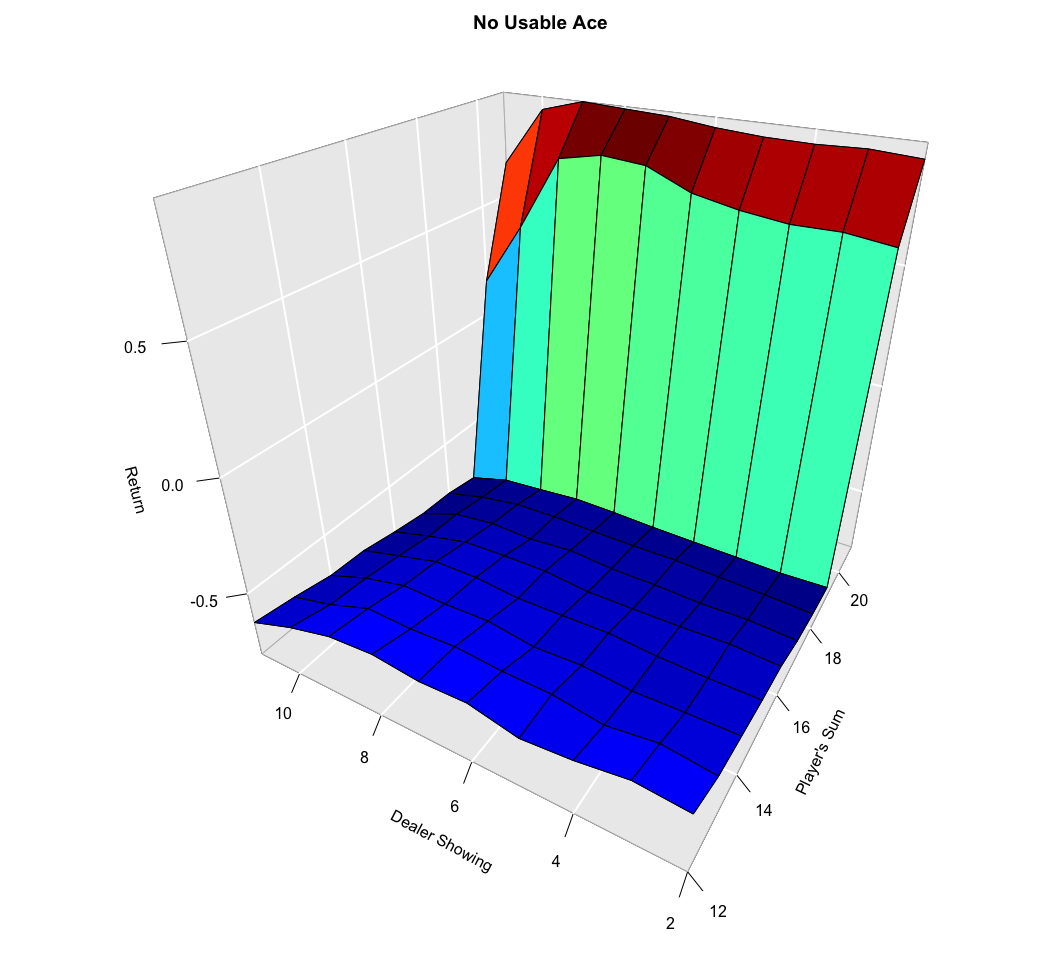
\includegraphics[width=12cm]{figures/q3-1.png}
\end{figure}

\begin{figure}[H]
  \centering
  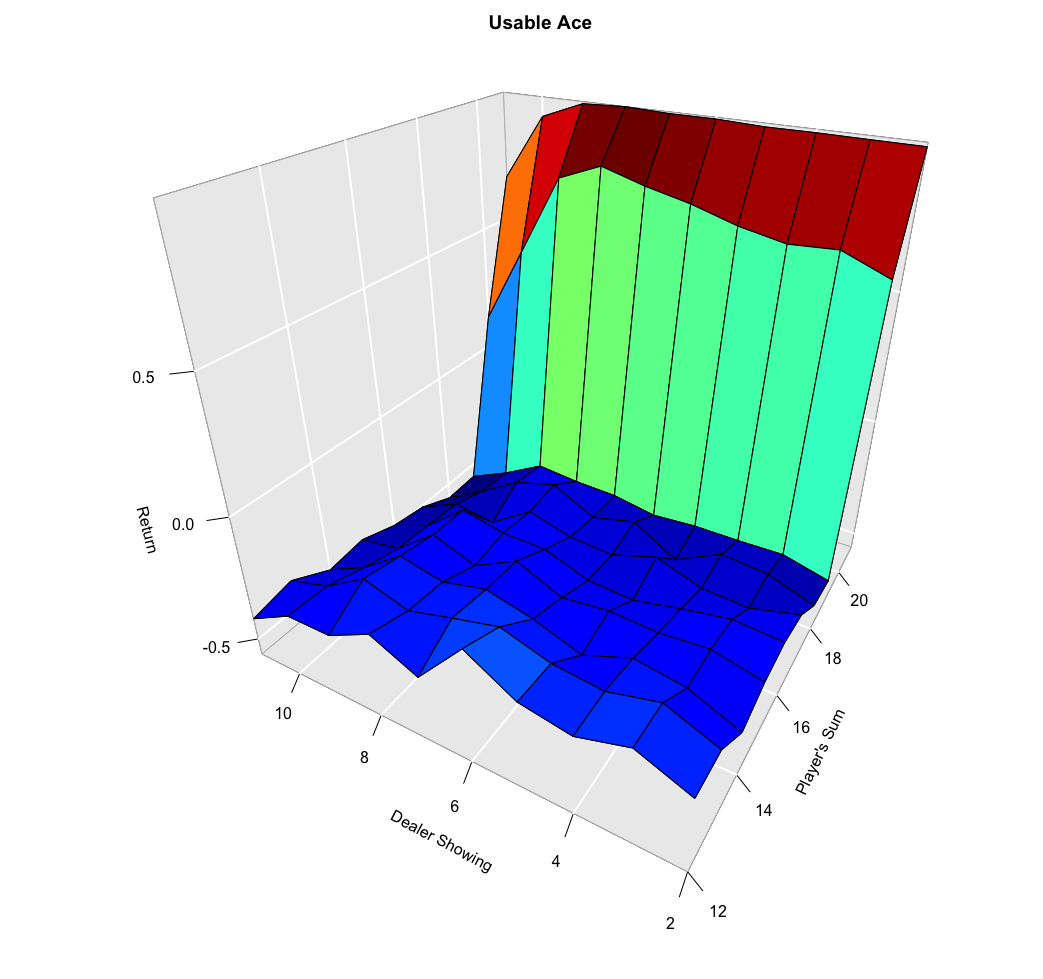
\includegraphics[width=12cm]{figures/q3-2.png}
\end{figure}

\end{document}